\section{Increasing System Performance}

\begin{concept}{Performance Optimization Trade-offs}
  \vspace{2mm}\\
\begin{tabular}{|l|l|}
\hline
\textbf{Optimizing for} & \textbf{Drawbacks on} \\
\hline
Higher speed & Power, cost, chip area \\
\hline
Lower cost & Speed, reliability \\
\hline
Zero power consumption & Speed, cost \\
\hline
Super reliable & Chip area, cost, speed \\
\hline
Temperature range & Power, cost, lifetime \\
\hline
\end{tabular}
\end{concept}

\begin{concept}{Instruction Set Architectures}\\
\textbf{RISC (Reduced Instruction Set Computer):}
\begin{itemize}
  \item Few instructions with uniform format
  \item Fast decoding, simple addressing
  \item Less hardware $\rightarrow$ higher clock rates
  \item More chip space for registers (up to 256)
  \item Load-store architecture reduces memory access
  \item CPU works at full speed on registers
  \item Enables shorter, efficient pipelines (instruction size/duration)
\end{itemize}

\textbf{CISC (Complex Instruction Set Computer):}
\begin{itemize}
  \item More complex and more instructions
  \item Lower memory usage for complex programs
  \item Potential performance gain for short programs
  \item More complex hardware required
\end{itemize}

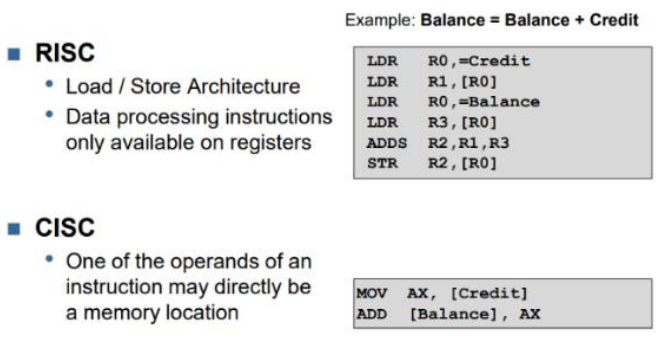
\includegraphics[width=\linewidth]{images/risc_cisc.png}
\end{concept}

\begin{definition}{Von Neumann Architectures}
\begin{itemize}
  \item Single memory for program and data
  \item Single bus system between CPU and memory
\end{itemize}

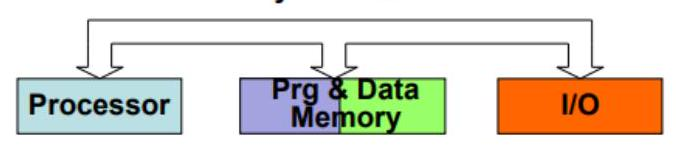
\includegraphics[width=0.7\linewidth]{images/2024_12_29_79e6b22f503fb7b4f718g-13}
\end{definition}

\begin{definition}{Harvard Architecture:}
\begin{itemize}
  \item Separate program and data memories
  \item Two sets of address/data buses
  \item Originally from Harvard Mark I
\end{itemize}

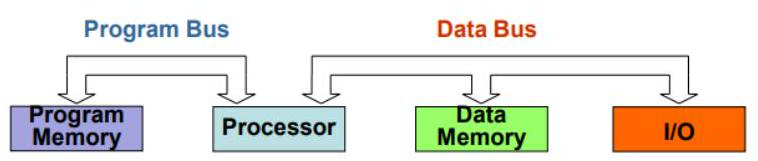
\includegraphics[width=0.7\linewidth]{images/2024_12_29_79e6b22f503fb7b4f718g-13(2)}
\end{definition}

\begin{theorem}{How to increase system speed?}\\
  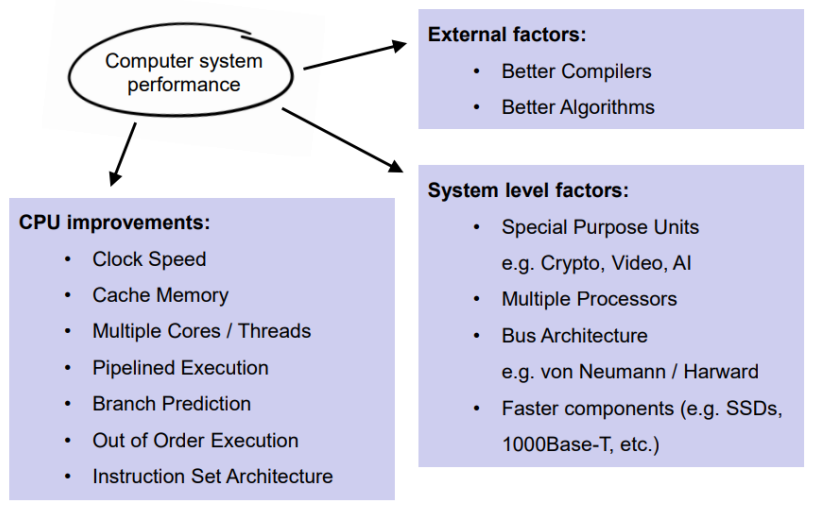
\includegraphics[width=\linewidth]{images/howtoincrease.png}
\end{theorem}

\subsubsection{Pipelining}

\begin{concept}{Sequential vs. Pipelined Execution}\\
\textbf{Sequential Execution:}\\
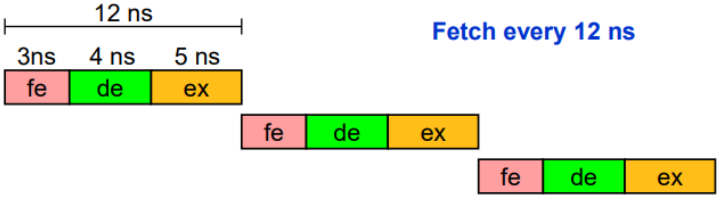
\includegraphics[width=\linewidth]{images/sequentialexec.png}

\textbf{Pipelined Execution:}\\
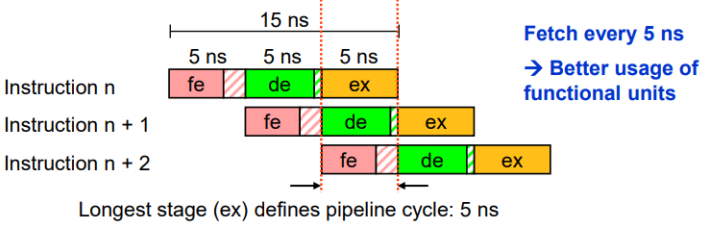
\includegraphics[width=\linewidth]{images/pipelinedexec.png}
\end{concept}

\begin{definition}{Pipelining}\\
Process of fetching next instruction while current one decodes:

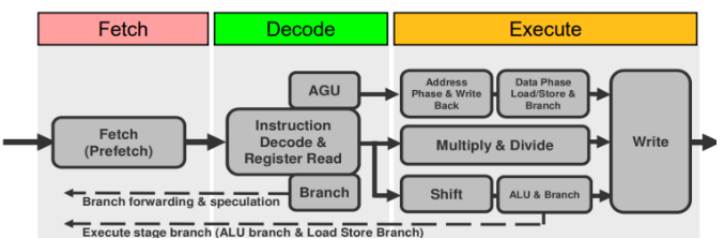
\includegraphics[width=\linewidth]{images/fetchwhiledecode.png}

\textbf{Advantages:}
\begin{itemize}
  \item Uniform execution time per stage
  \item Significant performance improvement
  \item Simpler hardware per stage allows higher clock rates
\end{itemize}

\textbf{Disadvantages:}
\begin{itemize}
  \item Blocking stages affect whole pipeline
  \item Possible Memory access conflicts between stages
\end{itemize}
\end{definition}

\begin{concept}{Pipeline Stages} (Example)
\begin{itemize}
  \item Fetch (Fe): Read instruction - 3ns
  \item Decode (De): Process instruction - 4ns
  \item Execute (Ex): Execute and writeback - 5ns
\end{itemize}

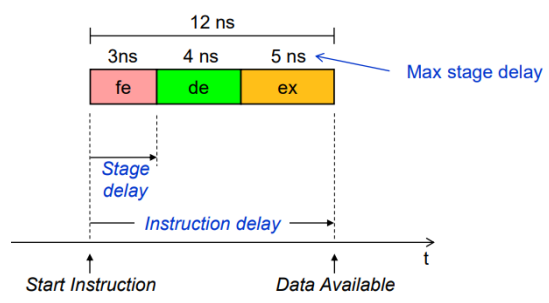
\includegraphics[width=0.8\linewidth]{images/pipelinestages.png}
\end{concept}

\begin{concept}{Pipeline Execution}\\
\textbf{Optimal Case:}
\begin{itemize}
  \item Register-only operations
  \item 6 instructions in 6 cycles
  \item CPI = 1 (Cycles Per Instruction)
\end{itemize}

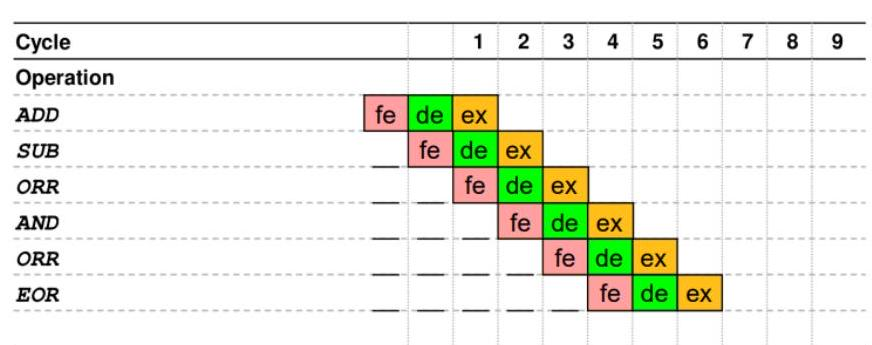
\includegraphics[width=\linewidth]{images/2024_12_29_79e6b22f503fb7b4f718g-14}

\textbf{LDR Special Case:}
\begin{itemize}
  \item 6 instructions in 7 cycles due to memory access
  \item Pipeline stalls for memory read
  \item CPI = 1.2
\end{itemize}

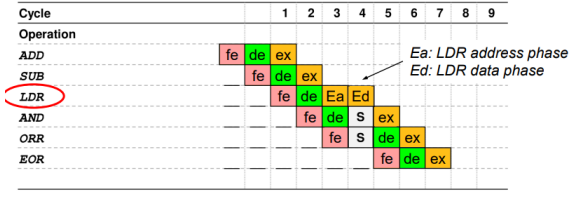
\includegraphics[width=\linewidth]{images/ldrpipelinespecialcase.png}
\end{concept}

\begin{corollary}{Pipeline important definitions}
\begin{itemize}
  \item \textbf{CPI}: Cycles per instruction
  \item \textbf{IPC}: Instructions per cycle
  \item \textbf{Fe, De, Ex}: Stage delays
  \item \textbf{Cycles}: Number of cycles for instruction
  \item \textbf{Performance}: $\frac{1}{\text{Total delay}}$
  \item \textbf{Throughput}: $\frac{1}{\text{Max stage delay}}$
  \item \textbf{Initial latency}: Number of cycles until pipeline is filled
  \item \textbf{Performance improvement}: $\frac{\text{Without pipeline delay}}{\text{With pipeline delay}}$
  \item \textbf{Pipeline stalls}: Delay due to memory access
\end{itemize}  
\end{corollary}


\begin{formula}{Pipeline Performance Calculation}\\
For a processor with n pipeline stages:

\textbf{Without pipelining:}
\begin{itemize}
  \item Time per instruction = Sum of all stage delays
  \item Performance (Instructions/Second) = $$\frac{1}{\text{Total delay}}$$
\end{itemize}

\textbf{With pipelining:}
\begin{itemize}
  \item Time per instruction = Longest stage delay
  \item Initial latency = n cycles
  \item Throughput (Instructions/Second) = $$\frac{1}{\text{Max stage delay}}$$
\end{itemize}

Note: Pipeline must be filled first! After filling, instructions are executed after every stage.
\end{formula}



\begin{KR}{Analyzing Pipeline Performance}\\
Steps for calculating pipeline performance:
\vspace{2mm}\\
\textbf{1. Calculate performance without pipelining:}
\begin{itemize}
  \item Total delay = Sum of all stage delays
  \item Performance = $\frac{1}{\text{Total delay}}$
\end{itemize}
Example for 3 stages:
    \begin{itemize}
      \item Fetch: 3ns, Decode: 4ns, Execute: 5ns
      \item Total delay = 12ns
      \item Performance = 83.3 MIPS
    \end{itemize}
\vspace{2mm}
\textbf{2. Calculate performance with pipelining:}
\begin{itemize}
  \item Critical path = Longest stage delay
  \item Initial latency = Number of stages
  \item Throughput = $\frac{1}{\text{Max stage delay}}$
\end{itemize}
Example for 3 stages:
    \begin{itemize}
      \item Max stage delay = 5ns (Execute)
      \item Initial latency = 3 cycles
      \item Throughput = 200 MIPS
    \end{itemize}
\vspace{2mm}
\textbf{3. Calculate performance improvement:}
$$\text{Improvement }=\frac{\text{Pipelined throughput}}{\text{Non-pipelined throughput}}$$
Example: $$\frac{200}{83.3} = 2.4\times \text{speedup}$$ 
\end{KR}

\begin{example2}{Pipeline Performance Calculation}
\begin{itemize}
  \item Stage delays: Fe=3ns, De=4ns, Ex=5ns
  \item Without pipeline: 12ns per instruction
  \item With pipeline: 5ns per instruction after filling
  \item Performance improvement: 2.4×
\end{itemize}
\end{example2}



\columnbreak

\begin{concept}{Pipeline Hazards and Optimization}\\
\textbf{Control Hazards:}
\begin{itemize}
  \item Branch/jump decisions in execute stage (stage 3)
  \item Worst case scenario: conditional branch taken
  \item Pipeline stalls for taken branches
\end{itemize}
\vspace{4mm}
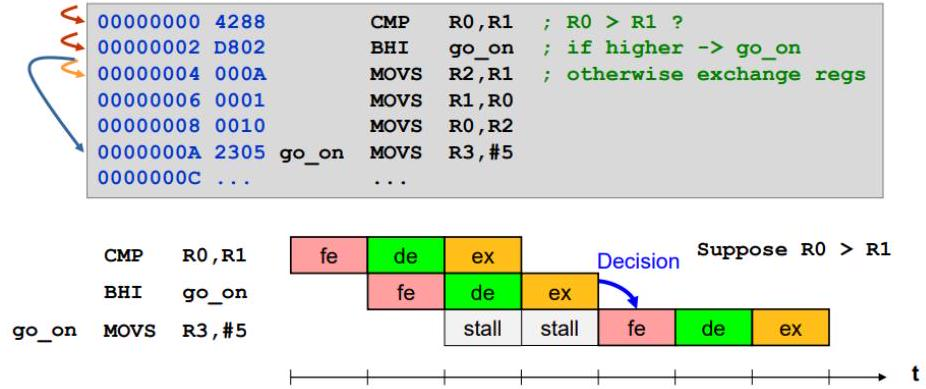
\includegraphics[width=\linewidth]{images/2024_12_29_79e6b22f503fb7b4f718g-15}\\

\textbf{Reduce control hazards:} Use loop fusion!
\end{concept}



\begin{example2}{Pipeline Hazard Analysis}

1. Structural Hazard:
\begin{lstlisting}[language=armasm, style=basesmol]
; Multiple instructions need memory access
LDR R0, [R1]    ; Load from memory
LDR R2, [R3]    ; Load from memory - must wait
; Pipeline stalls because memory system can't handle both loads
\end{lstlisting}

2. Data Hazard:
\begin{lstlisting}[language=armasm, style=basesmol]
ADDS R0, R1, R2  ; R0 gets new value
ADDS R3, R0, R4  ; Uses R0 before ready
; Second instruction must wait for first to complete
\end{lstlisting}

3. Control Hazard:
\begin{lstlisting}[language=armasm, style=basesmol]
CMP  R0, #0      ; Compare
BEQ  target      ; Branch if equal
ADD  R1, R2, R3  ; May be unnecessary
SUB  R4, R5, R6  ; May be unnecessary
target
; Pipeline must flush if branch taken
\end{lstlisting}
\end{example2}

\begin{corollary}{Pipeline Optimization}\\
\textbf{Optimization Techniques:}
\begin{itemize}
  \item Branch prediction based on history
  \begin{itemize}
    \item Store last decisions made for each conditional branch
    \\$\rightarrow$ probability is high that the same decision will be made again
  \end{itemize}
  \item Instruction prefetch
  \begin{itemize}
    \item Fetch several instructions in advance
    \\$\rightarrow$ reduces pipeline stalls
    \\$\rightarrow$ better use of system bus
    \\$\rightarrow$ possibility of ''Out-of-order execution''
  \end{itemize}
  \item Out-of-order execution
  \begin{itemize}
    \item If one instruction stalls, it might be possible to already execute next instruction
    \\$\rightarrow$ requires complex hardware
  \end{itemize}
\end{itemize}

\textbf{Optimization Limits:}
\begin{itemize}
  \item Complex optimizations $\rightarrow$ severe security problems 
  \item Instructions executed, that would throw access violations under ''In Order'' circumstances
  \item ''Meltdwon'' and ''Spectre'' attacks: allow process to access memory of other processes
\end{itemize}
\end{corollary}

\begin{KR}{Loop Optimization Techniques}\\
Steps for optimizing loops:

1. Loop Fusion:
\begin{lstlisting}[language=C, style=basesmol]
// Before optimization - two loops
for (i = 0; i < N; i++) {
    a[i] = b[i] * c[i];
}
for (i = 0; i < N; i++) {
    d[i] = a[i] + c[i];
}

// After fusion - single loop
for (i = 0; i < N; i++) {
    a[i] = b[i] * c[i];
    d[i] = a[i] + c[i];
}
\end{lstlisting}

2. Loop Unrolling:
\begin{lstlisting}[language=C, style=basesmol]
// Before unrolling
for (i = 0; i < N; i++) {
    sum += array[i];
}

// After unrolling by factor 4
for (i = 0; i < N-3; i += 4) {
    sum += array[i];
    sum += array[i+1];
    sum += array[i+2];
    sum += array[i+3];
}
// Handle remaining elements
for (; i < N; i++) {
    sum += array[i];
}
\end{lstlisting}

3. Memory Access Optimization:
\begin{itemize}
  \item Align data to cache line boundaries
  \item Use sequential memory access patterns
  \item Minimize cache misses
\end{itemize}
\end{KR}



\columnbreak

\subsubsection{Parallel Computing}

\begin{concept}{Parallel Computing}\\
Different approaches to parallelism:
\begin{itemize}
  \item \textbf{Streaming/Vector Processing}: Single instruction processes multiple data items simultaneously
  \item \textbf{Multithreading}: Multiple programs/threads share a single CPU
  \item \textbf{Multicore}: One processor with multiple CPU cores
  \item \textbf{Multiprocessor}: A computer system containing multiple processors
\end{itemize}
\end{concept}

\begin{example2}{Multicore vs Multiprocessor}
Key differences:
\begin{itemize}
  \item \textbf{Multicore}:
    \begin{itemize}
      \item Multiple CPU cores on single chip
      \item Shared cache and memory interface
      \item Lower communication overhead
      \item More power efficient
    \end{itemize}
  \item \textbf{Multiprocessor}:
    \begin{itemize}
      \item Multiple separate CPU chips
      \item Independent caches
      \item Higher communication overhead
      \item More scalable for large systems
    \end{itemize}
\end{itemize}
\end{example2}

\begin{example2}{Multi-Core Programming}
Example of parallel task processing:

\begin{lstlisting}[language=C, style=basesmol]
typedef struct {
    int *array;
    int start;
    int end;
    long sum;
} task_t;

void* partial_sum(void* arg) {
    task_t* task = (task_t*)arg;
    long sum = 0;
    
    for (int i = task->start; i < task->end; i++) {
        sum += task->array[i];
    }
    task->sum = sum;
    return NULL;
}
// Split work across multiple cores
void parallel_sum(int* array, int size, int num_cores) {
    task_t tasks[MAX_CORES];
    int chunk = size / num_cores;
    // Create tasks for each core
    for (int i = 0; i < num_cores; i++) {
        tasks[i].array = array;
        tasks[i].start = i * chunk;
        tasks[i].end = (i == num_cores-1) ? 
                      size : (i+1) * chunk;
        // Launch task on core i
        launch_on_core(i, partial_sum, &tasks[i]);
    }
    // Wait for all cores and combine results
    long total = 0;
    for (int i = 0; i < num_cores; i++) {
        wait_for_core(i);
        total += tasks[i].sum;
    }
    return total;
}
\end{lstlisting}
\end{example2}


\begin{concept}{Parallel Processing Models}\\
\textbf{SISD (Single Instruction Single Data):}
\begin{itemize}
  \item Traditional sequential processing
  \item One instruction processes one data item
  \item Example: Basic scalar processor
\end{itemize}

\textbf{SIMD (Single Instruction Multiple Data):}
\begin{itemize}
  \item Vector processing
  \item One instruction processes multiple data items
  \item Examples: MMX, SSE, AVX instructions
\end{itemize}

\textbf{MIMD (Multiple Instruction Multiple Data):}
\begin{itemize}
  \item True parallel processing
  \item Multiple processors execute different instructions
  \item Example: Multicore systems
\end{itemize}
\end{concept}



\begin{example2}{SIMD Operations}\\
Example of vectorized operations:

\begin{lstlisting}[language=C, style=basesmol]
// Scalar addition
void add_arrays_scalar(int *a, int *b, int *c, int n) {
    for (int i = 0; i < n; i++) {
        c[i] = a[i] + b[i];
    }
}

// SIMD/Vector addition (conceptual)
void add_arrays_vector(int *a, int *b, int *c, int n) {
    for (int i = 0; i < n; i += 4) {
        // Load 4 elements at once
        vector_t va = vector_load(&a[i]);
        vector_t vb = vector_load(&b[i]);
        // Add 4 pairs of elements simultaneously
        vector_t vc = vector_add(va, vb);
        // Store 4 results at once
        vector_store(&c[i], vc);
    }
}
\end{lstlisting}
\end{example2}

\subsubsection{Conclusion on Performance Optimization}



\begin{concept}{Performance Growth Overview}\\
Historical development:
\begin{itemize}
  \item Early improvements:
    \begin{itemize}
      \item Increasing clock frequencies
      \item Better manufacturing processes
      \item Smaller transistor sizes
    \end{itemize}
  \item Modern improvements:
    \begin{itemize}
      \item Advanced architectural concepts (RISC, Pipelining)
      \item Multiple cores
      \item Specialized hardware units
    \end{itemize}
  \item Current limitations:
    \begin{itemize}
      \item Power density
      \item Heat dissipation
      \item Memory wall
      \item Parallelization overhead
    \end{itemize}
\end{itemize}
\end{concept}

\begin{KR}{Optimizing System Performance}\\
Steps for performance optimization:
\begin{enumerate}
  \item Analyze performance bottlenecks
  \item Choose appropriate architecture:
    \begin{itemize}
      \item RISC vs CISC based on application
      \item Consider memory architecture
    \end{itemize}
  \item Implement pipelining:
    \begin{itemize}
      \item Balance stage delays
      \item Handle hazards appropriately
    \end{itemize}
  \item Consider parallelization options
  \item Evaluate security implications
\end{enumerate}
\end{KR}

\begin{corollary}{System Level Optimization}\\
Different approaches to improve performance:
\begin{itemize}
  \item \textbf{External Factors}:
    \begin{itemize}
      \item Better compiler optimization
      \item Improved algorithms
      \item Efficient software design
    \end{itemize}
  \item \textbf{System Level Factors}:
    \begin{itemize}
      \item Special Purpose Units (e.g., Crypto, Video)
      \item Multiple Processors
      \item Bus Architecture optimization
      \item Faster peripheral components
    \end{itemize}
  \item \textbf{CPU Improvements}:
    \begin{itemize}
      \item Increased Clock Speed
      \item Cache Memory
      \item Multiple Cores
      \item Pipeline Optimization
      \item Branch Prediction
      \item Out-of-Order Execution
    \end{itemize}
\end{itemize}
\end{corollary}

\begin{KR}{Performance Optimization Guidelines}\\
Steps for system optimization:

1. \textbf{Analyze Requirements}:
\begin{itemize}
  \item Performance targets
  \item Power constraints
  \item Cost limitations
  \item Reliability needs
\end{itemize}

2. \textbf{Choose Architecture}:
\begin{itemize}
  \item RISC vs CISC
  \item Memory architecture
  \item Pipeline depth
  \item Parallelization approach
\end{itemize}

3. \textbf{Optimize Implementation}:
\begin{itemize}
  \item Balance pipeline stages
  \item Implement hazard handling
  \item Consider branch prediction
  \item Optimize memory access
\end{itemize}

4. \textbf{Security Considerations}:
\begin{itemize}
  \item Evaluate optimization risks
  \item Consider side-channel attacks
  \item Balance performance and security
\end{itemize}
\end{KR}



